\documentclass{article}

\usepackage[preprint]{neurips_2026}
\makeatletter
\renewcommand{\@noticestring}{ESE 4020 (Statistics for Data Science) course project, University of Pennsylvania, Fall 2026. Written in the NeurIPS format; not peer reviewed.}
\makeatother

\usepackage[utf8]{inputenc}
\usepackage[T1]{fontenc}
\usepackage{hyperref}
\usepackage{url}
\usepackage{booktabs}
\usepackage{amsfonts,amsmath}
\usepackage{nicefrac}
\usepackage{microtype}
\usepackage{xcolor}
\usepackage{graphicx}
\usepackage{siunitx}
\sisetup{group-separator={,}}

% Auto-generated by src/make_numbers.py. Do not edit.
\newcommand{\gamesJan}{1{,}497{,}237}
\newcommand{\keptJan}{1{,}478{,}833}
\newcommand{\playersJan}{40{,}396}
\newcommand{\rmJanCorrespondence}{5{,}458}
\newcommand{\rmJanAbandoned}{11{,}708}
\newcommand{\rmJanMissingRating}{0}
\newcommand{\rmJanUnfinishedResult}{0}
\newcommand{\rmJanWrongMonthOrBadDate}{1{,}238}
\newcommand{\nJanClassical}{433{,}581}
\newcommand{\nJanBullet}{405{,}362}
\newcommand{\nJanBlitz}{639{,}890}
\newcommand{\gamesFeb}{1{,}495{,}553}
\newcommand{\keptFeb}{1{,}476{,}869}
\newcommand{\playersFeb}{40{,}645}
\newcommand{\rmFebCorrespondence}{6{,}498}
\newcommand{\rmFebAbandoned}{10{,}187}
\newcommand{\rmFebMissingRating}{1}
\newcommand{\rmFebUnfinishedResult}{0}
\newcommand{\rmFebWrongMonthOrBadDate}{1{,}998}
\newcommand{\nFebBullet}{391{,}126}
\newcommand{\nFebBlitz}{649{,}835}
\newcommand{\nFebClassical}{435{,}908}
\newcommand{\meanScoreJan}{0.519}
\newcommand{\drawPctJan}{3.7}
\newcommand{\sdGapJan}{205}
\newcommand{\betaOne}{0.00450}
\newcommand{\betaOneCI}{[0.00448, 0.00452]}
\newcommand{\slopeRatio}{0.78}
\newcommand{\slopeRatioCI}{[0.778, 0.786]}
\newcommand{\betaZero}{0.0667}
\newcommand{\advPts}{14.8}
\newcommand{\advPtsCI}{[14.1, 15.7]}
\newcommand{\advScorePct}{1.67}
\newcommand{\slopeBullet}{0.80}
\newcommand{\slopeBulletCI}{[0.79, 0.81]}
\newcommand{\advBullet}{13.4}
\newcommand{\advBulletCI}{[11.8, 14.9]}
\newcommand{\advScoreBullet}{1.54}
\newcommand{\slopeBlitz}{0.77}
\newcommand{\slopeBlitzCI}{[0.77, 0.78]}
\newcommand{\advBlitz}{15.8}
\newcommand{\advBlitzCI}{[14.8, 16.8]}
\newcommand{\advScoreBlitz}{1.76}
\newcommand{\slopeClassical}{0.77}
\newcommand{\slopeClassicalCI}{[0.76, 0.78]}
\newcommand{\advClassical}{14.9}
\newcommand{\advClassicalCI}{[13.5, 16.3]}
\newcommand{\advScoreClassical}{1.65}
\newcommand{\cvPooled}{0.61946}
\newcommand{\cvPooledSE}{0.00044}
\newcommand{\cvPooledDiff}{+0.11}
\newcommand{\cvPooledDiffSE}{0.13}
\newcommand{\cvBase}{0.61945}
\newcommand{\cvBaseSE}{0.00043}
\newcommand{\cvBaseDiff}{+0.00}
\newcommand{\cvBaseDiffSE}{0.00}
\newcommand{\cvRating}{0.61942}
\newcommand{\cvRatingSE}{0.00043}
\newcommand{\cvRatingDiff}{-0.26}
\newcommand{\cvRatingDiffSE}{0.08}
\newcommand{\cvSpline}{0.61927}
\newcommand{\cvSplineSE}{0.00044}
\newcommand{\cvSplineDiff}{-1.79}
\newcommand{\cvSplineDiffSE}{0.18}
\newcommand{\cvGbm}{0.61913}
\newcommand{\cvGbmSE}{0.00044}
\newcommand{\cvGbmDiff}{-3.22}
\newcommand{\cvGbmDiffSE}{0.31}
\newcommand{\splineDf}{12}
\newcommand{\gbmTrees}{100}
\newcommand{\gbmLeaves}{127}
\newcommand{\gbmRate}{0.05}
\newcommand{\nLogitConfigs}{26}
\newcommand{\nGbmConfigs}{20}
\newcommand{\teEloLL}{0.6265}
\newcommand{\teEloLLCI}{[0.6256, 0.6274]}
\newcommand{\teEloBrier}{0.2089}
\newcommand{\teEloBrierCI}{[0.2085, 0.2092]}
\newcommand{\teEloVsBase}{+45.0}
\newcommand{\teEloVsBaseCI}{[+43.1, +46.9]}
\newcommand{\teEloVsElo}{+0.0}
\newcommand{\teEloVsEloCI}{[+0.0, +0.0]}
\newcommand{\teFloorLL}{0.6924}
\newcommand{\teFloorLLCI}{[0.6924, 0.6925]}
\newcommand{\teFloorBrier}{0.2403}
\newcommand{\teFloorBrierCI}{[0.2402, 0.2404]}
\newcommand{\teFloorVsBase}{+704.5}
\newcommand{\teFloorVsBaseCI}{[+696.9, +712.6]}
\newcommand{\teFloorVsElo}{+659.5}
\newcommand{\teFloorVsEloCI}{[+650.6, +669.2]}
\newcommand{\tePooledLL}{0.6220}
\newcommand{\tePooledLLCI}{[0.6212, 0.6228]}
\newcommand{\tePooledBrier}{0.2076}
\newcommand{\tePooledBrierCI}{[0.2073, 0.2079]}
\newcommand{\tePooledVsBase}{+0.3}
\newcommand{\tePooledVsBaseCI}{[+0.2, +0.5]}
\newcommand{\tePooledVsElo}{-44.6}
\newcommand{\tePooledVsEloCI}{[-46.5, -42.8]}
\newcommand{\teBaseLL}{0.6220}
\newcommand{\teBaseLLCI}{[0.6212, 0.6227]}
\newcommand{\teBaseBrier}{0.2076}
\newcommand{\teBaseBrierCI}{[0.2073, 0.2079]}
\newcommand{\teBaseVsBase}{+0.0}
\newcommand{\teBaseVsBaseCI}{[+0.0, +0.0]}
\newcommand{\teBaseVsElo}{-45.0}
\newcommand{\teBaseVsEloCI}{[-46.9, -43.1]}
\newcommand{\teSplineLL}{0.6218}
\newcommand{\teSplineLLCI}{[0.6210, 0.6226]}
\newcommand{\teSplineBrier}{0.2076}
\newcommand{\teSplineBrierCI}{[0.2072, 0.2079]}
\newcommand{\teSplineVsBase}{-1.7}
\newcommand{\teSplineVsBaseCI}{[-2.1, -1.3]}
\newcommand{\teSplineVsElo}{-46.7}
\newcommand{\teSplineVsEloCI}{[-48.8, -44.6]}
\newcommand{\teGbmLL}{0.6217}
\newcommand{\teGbmLLCI}{[0.6209, 0.6224]}
\newcommand{\teGbmBrier}{0.2075}
\newcommand{\teGbmBrierCI}{[0.2072, 0.2078]}
\newcommand{\teGbmVsBase}{-3.2}
\newcommand{\teGbmVsBaseCI}{[-3.7, -2.7]}
\newcommand{\teGbmVsElo}{-48.2}
\newcommand{\teGbmVsEloCI}{[-50.4, -46.2]}
\newcommand{\calElo}{0.0304}
\newcommand{\calBase}{0.0039}
\newcommand{\calSpline}{0.0027}
\newcommand{\calGbm}{0.0025}
\newcommand{\calRatio}{8}
\newcommand{\freqSlopeTen}{0.80}
\newcommand{\freqShareTen}{96}
\newcommand{\freqSlopeThirty}{0.81}
\newcommand{\freqShareThirty}{89}
\newcommand{\freqSlopeHundred}{0.82}
\newcommand{\freqShareHundred}{67}
\newcommand{\prevTwentyShare}{67}
\newcommand{\prevTwentyDisp}{0.82}
\newcommand{\prevTwentySmooth}{0.75}
\newcommand{\prevTwentyBothD}{0.62}
\newcommand{\prevTwentyBothPrev}{0.25}
\newcommand{\prevTwentySum}{0.87}
\newcommand{\prevTwentyCorr}{0.86}
\newcommand{\prevHundredShare}{33}
\newcommand{\prevHundredDisp}{0.83}
\newcommand{\prevHundredSmooth}{0.78}
\newcommand{\prevHundredBothD}{0.59}
\newcommand{\prevHundredBothPrev}{0.30}
\newcommand{\prevHundredSum}{0.89}
\newcommand{\prevHundredCorr}{0.87}
\newcommand{\simSigmaAll}{56}
\newcommand{\simSigmaFreq}{50}
\newcommand{\simSlopeFifty}{0.82}
\newcommand{\simAdvFifty}{14.6}
\newcommand{\simAdvTrue}{11.6}
\newcommand{\simDilutionFifty}{0.88}
\newcommand{\simScoreBiasFifty}{3}
\newcommand{\bandSlopeLow}{0.75}
\newcommand{\bandSlopeHigh}{0.84}
\newcommand{\bandSlopeHighCI}{[0.83, 0.85]}
\newcommand{\bandAdvScoreMin}{1.6}
\newcommand{\bandAdvScoreMax}{1.9}
\newcommand{\bandDrawLow}{3.0}
\newcommand{\bandDrawHigh}{5.0}
\newcommand{\sensForfeitSlope}{0.78}
\newcommand{\sensForfeitAdv}{18.0}
\newcommand{\sensForfeitAdvCI}{[17.1, 19.0]}
\newcommand{\sensForfeitShare}{67}
\newcommand{\sensDefaultSlope}{0.80}
\newcommand{\sensDefaultAdv}{14.3}
\newcommand{\sensDefaultAdvCI}{[13.5, 15.1]}
\newcommand{\sensDefaultShare}{98}
\newcommand{\sensGapSlope}{0.80}
\newcommand{\sensGapAdv}{14.4}
\newcommand{\sensGapAdvCI}{[13.7, 15.2]}
\newcommand{\sensGapShare}{94}
\newcommand{\sensInfractionSlope}{0.78}
\newcommand{\sensInfractionAdv}{14.8}
\newcommand{\sensInfractionAdvCI}{[14.1, 15.6]}
\newcommand{\sensInfractionShare}{100}
\newcommand{\sensFirstHalfSlope}{0.78}
\newcommand{\sensFirstHalfAdv}{14.5}
\newcommand{\sensFirstHalfAdvCI}{[13.4, 15.6]}
\newcommand{\sensFirstHalfShare}{47}
\newcommand{\sensSecondHalfSlope}{0.78}
\newcommand{\sensSecondHalfAdv}{15.1}
\newcommand{\sensSecondHalfAdvCI}{[14.0, 16.2]}
\newcommand{\sensSecondHalfShare}{53}
\newcommand{\eloGain}{45}
\newcommand{\splineGain}{1.7}
\newcommand{\gbmGain}{3.2}
\newcommand{\ratioGbm}{14}
\newcommand{\ratioSpline}{27}
\newcommand{\maxEloMiss}{0.08}
\newcommand{\maxFitMiss}{0.014}
\newcommand{\advSpread}{2.4}
\newcommand{\nInfraction}{101}
\newcommand{\nForfeitPct}{33}
\newcommand{\testGames}{1{,}476{,}869}
\newcommand{\slopeGapPct}{22}


\title{Is the Elo Formula Overconfident on Lichess?\\Rating Calibration and White's Advantage in 3 Million Games}

\author{%
  Liam Campbell \And Xinran Gao \And Pedro S\'anchez-Gil Galindo \\
  University of Pennsylvania
}

\begin{document}

\maketitle

\begin{abstract}
Do Lichess rating gaps predict game outcomes as well as the Elo expected-score formula claims, and how large is White's advantage across rating levels and time controls? We fit logistic regression by maximum likelihood to \keptJan{} rated games from January 2015, select models by 5-fold cross-validation over contiguous blocks of days, and score every model once on \keptFeb{} games from February 2015, with day-level bootstrap intervals. The fitted slope is \slopeRatio{} times Elo's $\ln(10)/400$ (95\% CI \slopeRatioCI), so the formula overstates the stronger player's score by up to \maxEloMiss; refitting cuts February log-loss by \eloGain{} units of $10^{-4}$ and the calibration error by a factor of \calRatio. Splines and gradient boosting add only \splineGain{} and \gbmGain{} units more. White's edge is \bandAdvScoreMin--\bandAdvScoreMax{} percentage points of expected score at equal ratings, nearly constant across rating bands and time controls. Rating noise could explain the shallow slope: a simulation with known truth shows that per-player noise of about \simSigmaAll{} rating points reproduces it, and smoothing each player's rating with his earlier games raises the combined slope to \prevTwentySum. Elo is overconfident as applied to displayed ratings, but our data cannot tell whether it is also wrong about true strength.
\end{abstract}

\section{Introduction}
\label{sec:intro}

Every online chess game is paired and scored with a rating system that converts a rating gap into an expected score. The Elo formula \citep{elo1978} sets White's expected score to
\begin{equation}
  E[S \mid d] \;=\; \frac{1}{1 + e^{-(\beta_0 + \beta_1 d)}}, \qquad \beta_0 = 0, \quad \beta_1 = \frac{\ln 10}{400} \approx 0.00576,
  \label{eq:elo}
\end{equation}
where $S \in \{1, \tfrac12, 0\}$ is White's score and $d$ is White's rating minus Black's. The formula fixes both parameters in advance: White gets no edge, and a 400-point gap means a 10-to-1 expected-score ratio. Players see these expectations every time they pick an opponent, and rating updates move in proportion to the gap between the result and the expectation.

We ask whether Lichess outcomes agree with \eqref{eq:elo}, and how large White's advantage is across rating levels and time controls. Treating \eqref{eq:elo} as a logistic regression with fixed coefficients makes the question testable: fit $\beta_0$ and $\beta_1$ by maximum likelihood and compare. A slope below $0.00576$ means the formula is overconfident; $\beta_0 > 0$ measures White's edge.

Our contributions are:
\begin{itemize}
  \item A careful calibration test of the Elo formula on \keptJan{} games, with folds and bootstrap resampling at the level of days, because players recur within a day. The fitted slope is \slopeRatio{} times Elo's (CI \slopeRatioCI), consistent across time controls.
  \item A held-out comparison on February 2015, scored once, of Elo, a constant floor, logistic regression, splines and gradient boosting. Refitting two parameters captures almost all of the available gain; more flexible models add little.
  \item Estimates of White's advantage that are robust to rating noise: about \advScorePct{} percentage points of expected score, flat across rating bands.
  \item Two checks on whether the shallow slope reflects noisy ratings rather than a wrong formula: a simulation with known truth and a smoothed-rating test. Both say noise of realistic size could explain much or all of it.
\end{itemize}

\section{Related work}
\label{sec:related}

\textbf{Rating systems.} Elo's model \citep{elo1978} is a logistic Bradley--Terry model \citep{bradley1952} with a fixed scale. Glicko \citep{glickman1999} and Glicko-2 \citep{glickman2001} add a rating deviation (RD) that tracks how uncertain each rating is; Lichess uses Glicko-2 and marks a rating provisional when its RD exceeds 110 points \citep{lichessfaq}. The public data omit RD, so the Elo formula is the natural parameter-free prediction from displayed ratings. \citet{sonas2002} argued that a linear expected-score curve fits FIDE results better than Elo's, and \citet{sonas2011}, analysing about 1.5 million FIDE games, found that actual results match about five-sixths of the rating gap, a flatter curve in line with ours. \citet{regan2011} rate play by move quality rather than results. We are not aware of a comparable held-out study on online games at this scale.

\textbf{Calibration, scoring and validation.} We score probabilistic predictions with log-loss and the Brier score, both strictly proper \citep{brier1950,gneiting2007}, and display calibration with reliability-style plots \citep{guo2017}. Model selection uses $K$-fold cross-validation \citep{hastie2009}; because fold scores are correlated, naive CV standard errors are too small \citep{bates2024}, so our claims rest on a day-level bootstrap \citep{efron1993} and an untouched test month.

\textbf{Measurement error.} Noise in a predictor biases a fitted slope toward zero (attenuation) in linear and nonlinear models alike \citep{carroll2006}. A displayed rating is a noisy estimate of strength, so a shallow fitted slope is ambiguous. We address this with a simulation and with a smoothed-rating test (Section~\ref{sec:method}).

\section{Data}
\label{sec:data}

We use the Lichess open database \citep{lichessdb} of standard rated games, released under CC0 1.0. January 2015 (\gamesJan{} games) is for fitting and model selection; February 2015 (\gamesFeb{} games) is the test set. We read only the PGN headers: the two ratings, the result, the event and clock (for the time control: bullet, blitz or classical), the termination, and the date. In order, we drop correspondence games (\rmJanCorrespondence{} in January), abandoned games (\rmJanAbandoned), games missing a rating (\rmJanMissingRating) and games dated in the previous month (\rmJanWrongMonthOrBadDate). This leaves \keptJan{} January games (bullet \nJanBullet, blitz \nJanBlitz, classical \nJanClassical) and \keptFeb{} February games. White's mean score is \meanScoreJan{} and \drawPctJan\% of games are draws. Usernames are mapped to integers in memory only to count each player's games and compute earlier-day mean ratings (Section~\ref{sec:noise}), then discarded; none is stored.

\section{Method}
\label{sec:method}

\textbf{Model and fitting.} We fit \eqref{eq:elo} and its extensions by maximum likelihood (course Section 3C), minimizing the mean negative log-likelihood
$-\tfrac1N\sum_i [S_i \log p_i + (1 - S_i)\log(1 - p_i)]$ with $p_i = \sigma(\theta^\top x_i)$. A draw has $S_i = \tfrac12$, which equals entering it as a win and a loss with weight $\tfrac12$ each. We use Newton's method; the gradient is $\sum_i (p_i - S_i)x_i$.

\textbf{Model ladder.} (1) \emph{Pooled}: $x = (1, d)$. (2) \emph{Baseline}: separate $\beta_0$ and $\beta_1$ for each time control. (3) Adds the mean rating $\bar r$ of the two players, $\bar r^2$ and $d\,\bar r$. (4) Adds a natural cubic spline in $d$ \citep{hastie2009} with $\{4,6,8,10,12\}$ knots at training-fold quantiles. Levels 3 and 4 carry a ridge penalty $\lambda \in \{0, 10^{-5}, 10^{-4}, 10^{-3}\}$ on standardized inputs. As a comparison from later in the course we fit gradient-boosted trees \citep{friedman2001,ke2017} (scikit-learn's histogram implementation, \citealp{pedregosa2011}) on $(d, \bar r, \text{time control})$, monotone increasing in $d$, with \nGbmConfigs{} settings of trees, leaves and learning rate. The two fixed references are the Elo formula and a floor that always predicts the training month's mean score.

\textbf{Validation.} All selection uses January only, by 5-fold cross-validation (course Section 4A) with each fold a contiguous block of days (1--7, 8--13, 14--19, 20--25, 26--31). Splitting by day matters because a player's games on one day are not independent. Spline knots, standardization and the floor are learned inside each training fold. The CV loss is the fold-size-weighted mean of the fold log-losses. We pick the lowest-CV logistic model and the lowest-CV boosted model, refit both on all of January, and score every model once on February. The test set is read by a single script that runs only after the selection is frozen and logs each run.

\textbf{Error bars.} We resample whole days with replacement \citep{efron1993} ($B = 2000$, seed 4020): the 31 January days for coefficients and the 28 February days for test scores and their paired differences. All intervals are 95\% percentile intervals. We report White's advantage both in rating points, $\beta_0/\beta_1$, and in expected score at $d = 0$, $\sigma(\beta_0) - \tfrac12$.

\textbf{Is it noise?} \label{sec:noise}
Three checks, all on January. (i) \emph{Frequent players}: refit on games where both players have many games that month, whose ratings should be better settled. (ii) \emph{Smoothed ratings}: for a game on day $t$, average each player's displayed ratings over his games on days $1,\dots,t-1$. This uses only the past, so it cannot contain the game's result, and it averages out short-term fluctuation. Regressing on both the displayed gap $d$ and the smoothed gap $d_{\text{prev}}$ asks whether the past carries information about strength beyond the current rating, which it should not if the displayed rating were exact. (iii) \emph{Simulation with known truth}: outcomes follow \eqref{eq:elo} exactly in true strength, with $\beta_0$ set to our estimate. Each displayed rating adds independent noise $N(0, \sigma^2)$, the true-gap variance is reduced so that the observed gap keeps January's distribution, and draws occur at the observed rate. For each $\sigma$ we fit the pooled model to \keptJan{} simulated games, 20 seeds.

\section{Results}
\label{sec:results}

\begin{figure}[t]
  \centering
  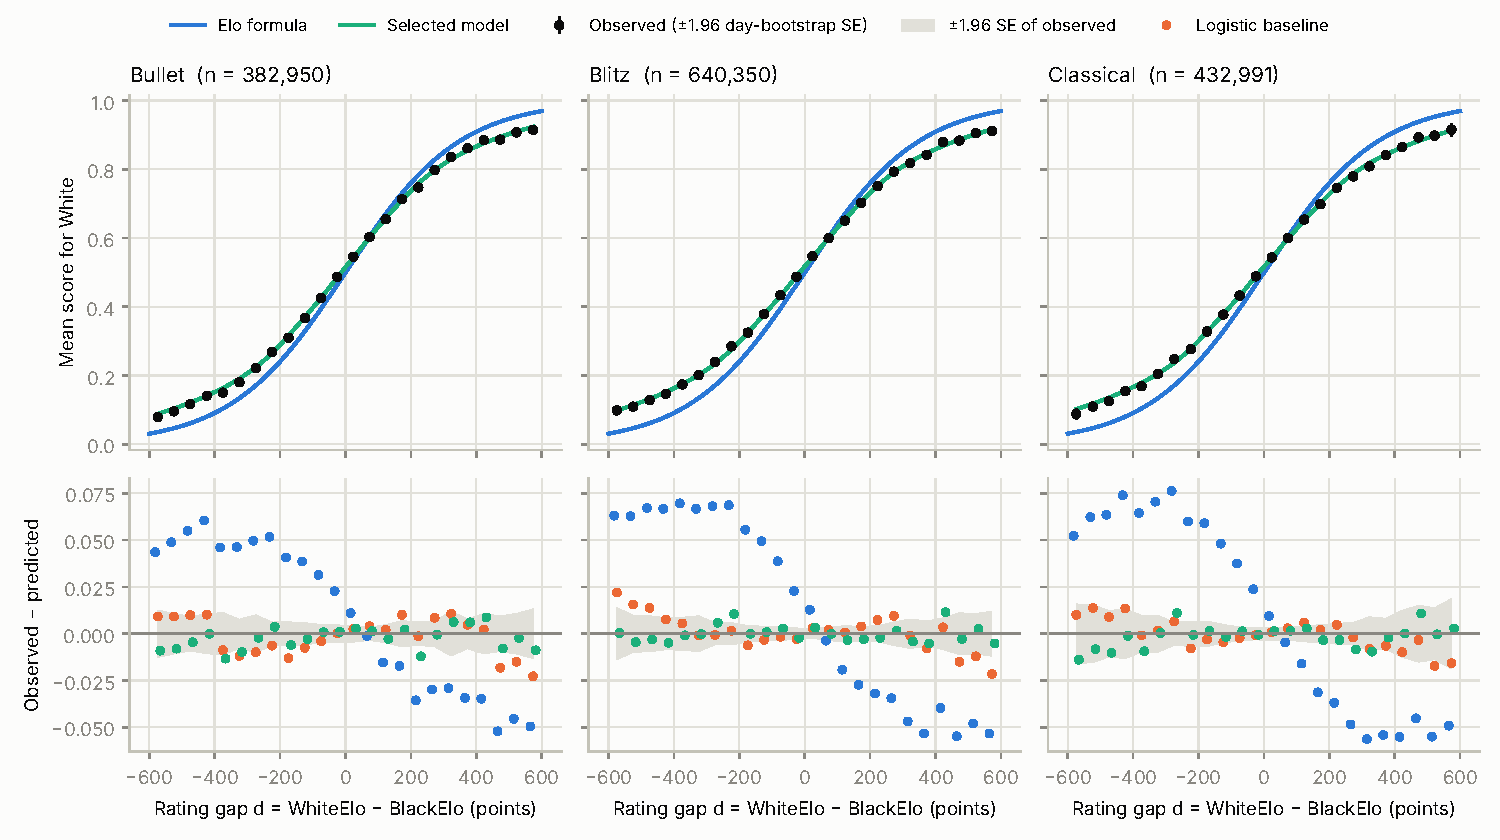
\includegraphics[width=\linewidth]{../figures/key_figure.pdf}
  \caption{\textbf{Elo's curve is too steep; a refitted logistic curve is not.} February 2015 (held out), games in 50-point bins of rating gap, by time control. Top: White's observed mean score with $\pm1.96$ day-bootstrap SE, the Elo formula and the selected model (logistic regression with a spline in $d$, fitted on January). Bottom: observed minus predicted for Elo, the logistic baseline and the selected model; the gray band is $\pm1.96$ SE of the observed mean. Elo overstates the stronger side by up to \maxEloMiss{} in every time control.}
  \label{fig:key}
\end{figure}

\begin{table}[t]
  \caption{\textbf{Every fitted model beats Elo by a wide margin; flexible models add little.} January: 5-fold day-blocked CV log-loss. February: test log-loss and Brier score with 95\% day-bootstrap intervals, the paired difference from the baseline in units of $10^{-4}$ (negative is better), and the mean absolute calibration error over the bins of Figure~\ref{fig:key}.}
  \label{tab:main}
  \centering
  \small
  \begin{tabular}{lcccccc}
    \toprule
    & CV & \multicolumn{5}{c}{February 2015 (test, scored once)} \\
    \cmidrule(lr){2-2}\cmidrule(lr){3-7}
    Model & log-loss & log-loss & 95\% CI & Brier & $\Delta$ vs.\ baseline & Calib.\ err. \\
    \midrule
    Mean-score floor & -- & \teFloorLL & \teFloorLLCI & \teFloorBrier & \teFloorVsBase{} \teFloorVsBaseCI & -- \\
    Elo formula & -- & \teEloLL & \teEloLLCI & \teEloBrier & \teEloVsBase{} \teEloVsBaseCI & \calElo \\
    Logit, pooled & \cvPooled & \tePooledLL & \tePooledLLCI & \tePooledBrier & \tePooledVsBase{} \tePooledVsBaseCI & -- \\
    Logit by time control (baseline) & \cvBase & \teBaseLL & \teBaseLLCI & \teBaseBrier & 0 & \calBase \\
    + spline in $d$ (\splineDf{} knots) & \cvSpline & \teSplineLL & \teSplineLLCI & \teSplineBrier & \teSplineVsBase{} \teSplineVsBaseCI & \calSpline \\
    Gradient boosting & \cvGbm & \teGbmLL & \teGbmLLCI & \teGbmBrier & \teGbmVsBase{} \teGbmVsBaseCI & \calGbm \\
    \bottomrule
  \end{tabular}
\end{table}

\textbf{Elo is overconfident on displayed ratings.} On January, the two-parameter fit gives $\hat\beta_1 = \betaOne$ \betaOneCI, \slopeRatio{} times Elo's slope (CI \slopeRatioCI); the interval is far from 1. The ratio is \slopeBullet{} (bullet), \slopeBlitz{} (blitz) and \slopeClassical{} (classical). Figure~\ref{fig:key} shows the consequence on February: the favorite scores up to \maxEloMiss{} less than Elo predicts and the underdog correspondingly more, and the refitted curves track the data within their error bars. Table~\ref{tab:main} puts numbers on it. The logistic baseline beats Elo by \eloGain{} units of $10^{-4}$ in log-loss, its interval far from zero, and cuts the calibration error from \calElo{} to \calBase. With \testGames{} test games almost every difference clears its interval, so we also judge size: the spline improves on the baseline by \splineGain{} units and gradient boosting by \gbmGain, both real but \ratioGbm{} to \ratioSpline{} times smaller than the gain from refitting Elo's two parameters. The CV ranking (Appendix~\ref{app:cv}) matched the test ranking. Separate slopes per time control are a tie with one pooled slope (CV difference \cvPooledDiff{} $\pm$ \cvPooledDiffSE{} units).

\begin{figure}[t]
  \centering
  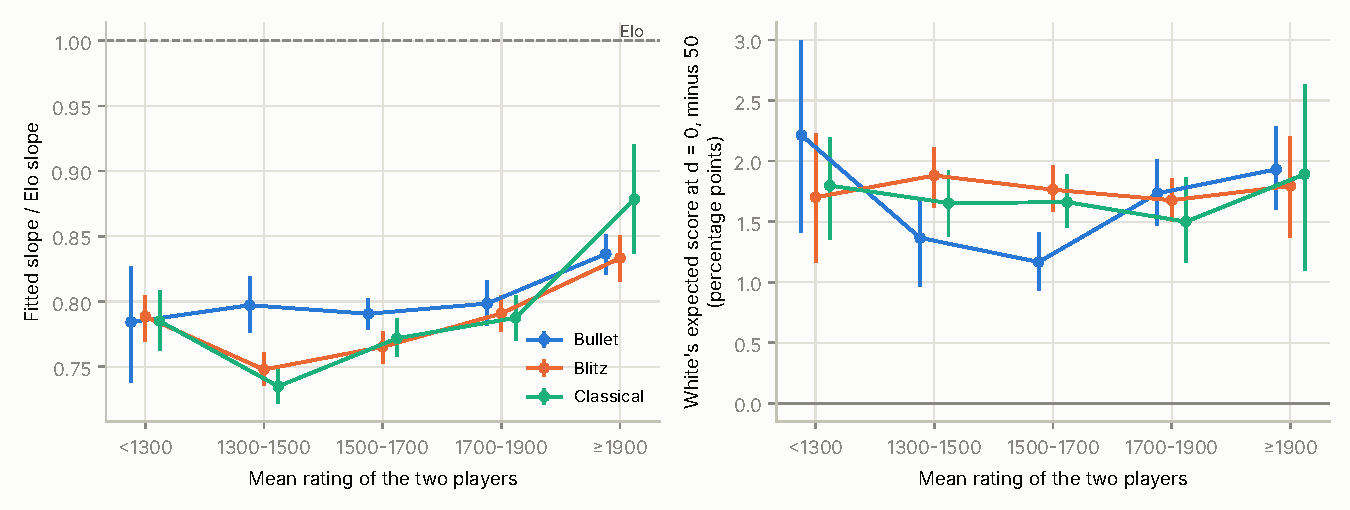
\includegraphics[width=\linewidth]{../figures/rating_bands.pdf}
  \caption{\textbf{The slope rises with rating level; White's edge does not.} January, two-parameter fits within bands of the players' mean rating, by time control, with 95\% day-bootstrap intervals ($B = 1000$). Left: fitted slope relative to Elo. Right: White's expected score at equal ratings minus 50\%.}
  \label{fig:bands}
\end{figure}

\textbf{White's advantage is small and stable.} Pooled, $\beta_0/\beta_1 = \advPts$ rating points \advPtsCI: about \advScorePct{} percentage points of expected score at equal ratings. By time control it is \advBullet{} \advBulletCI{} (bullet), \advBlitz{} \advBlitzCI{} (blitz) and \advClassical{} \advClassicalCI{} (classical) points; these differences span \advSpread{} points, which is practically small. Across rating bands (Figure~\ref{fig:bands}, right), White's edge stays between \bandAdvScoreMin{} and \bandAdvScoreMax{} percentage points. The slope, in contrast, rises with rating, from \bandSlopeLow{} to \bandSlopeHigh{} \bandSlopeHighCI{} times Elo above 1900 (left), as draws become more common (from \bandDrawLow\% to \bandDrawHigh\%).

\begin{figure}[t]
  \centering
  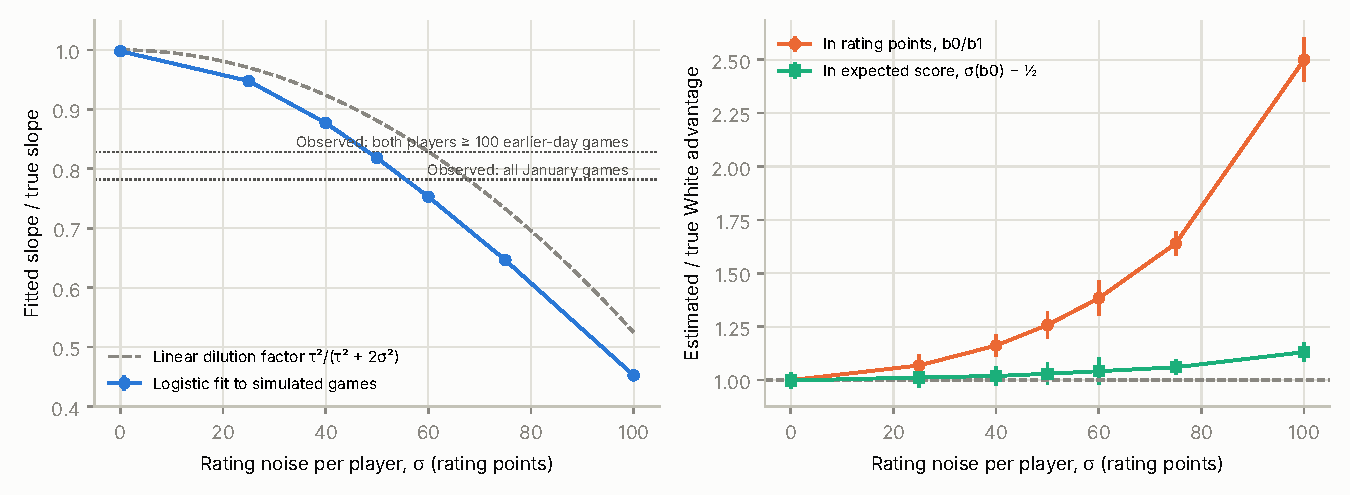
\includegraphics[width=\linewidth]{../figures/simulation_noise.pdf}
  \caption{\textbf{Realistic rating noise reproduces the shallow slope and inflates White's advantage in rating points, but not in expected score.} Simulation with known truth: outcomes follow the Elo curve exactly in true strength; displayed ratings add per-player noise $\sigma$. Left: fitted over true slope (20 seeds, $\pm1.96$ SD), with the linear dilution factor and our two observed slopes. Right: estimated over true White advantage in rating points ($\beta_0/\beta_1$) and in expected score ($\sigma(\beta_0) - \tfrac12$).}
  \label{fig:sim}
\end{figure}

\textbf{Could rating noise explain the shallow slope?} Restricting to games where both players have at least 10, 30 or 100 January games (\freqShareTen\%, \freqShareThirty\% and \freqShareHundred\% of games) raises the slope only to \freqSlopeTen, \freqSlopeThirty{} and \freqSlopeHundred{} times Elo. That alone would suggest a genuinely flatter curve. The simulation (Figure~\ref{fig:sim}, left) says otherwise: noise of $\sigma \approx \simSigmaFreq$ rating points per player already yields a slope of \simSlopeFifty, and $\sigma \approx \simSigmaAll$ reproduces the full-sample \slopeRatio. For a logistic curve and heavy-tailed gaps the attenuation is stronger than the linear dilution factor suggests. Noise of this size is plausible next to Lichess's 110-point provisional threshold \citep{lichessfaq}. The smoothed-rating test points the same way. On the \prevTwentyShare\% of games where both players have at least 20 earlier-day games, the smoothed gap alone has a lower slope than the displayed gap (\prevTwentySmooth{} vs.\ \prevTwentyDisp{} times Elo), as a lagging average should. Used together, however, both carry weight (\prevTwentyBothD{} and \prevTwentyBothPrev), and the combined slope rises to \prevTwentySum{} times Elo. The past thus holds information about strength that the displayed rating lacks, which is what noisy ratings imply, and a better estimate of strength closes a third or more of the gap to Elo. Noise also inflates White's advantage in rating points: at $\sigma = 50$ the simulation estimates \simAdvFifty{} points against a true \simAdvTrue{} (Figure~\ref{fig:sim}, right), while the advantage in expected score is off by only about \simScoreBiasFifty\%. This is why we report White's edge in score units.

\textbf{Robustness.} Dropping the \nInfraction{} games ended by a rules infraction changes nothing. Dropping games involving a rating of exactly 1500, the default for new accounts, raises the slope to \sensDefaultSlope, consistent with provisional ratings adding noise. Restricting to $|d| < 400$ gives \sensGapSlope. Dropping time-forfeit games leaves the slope unchanged but raises White's advantage to \sensForfeitAdv{} \sensForfeitAdvCI{} points, so White's edge is larger in games decided on the board. The two halves of January agree (Appendix~\ref{app:sens}).

\section{Discussion and limitations}
\label{sec:discussion}

The practical conclusion is firm: applied to displayed Lichess ratings in 2015, the Elo formula's slope is \slopeGapPct\% too steep and it ignores a White edge of about \advScorePct{} percentage points of expected score. Refitting two parameters removes almost all of the measurable miscalibration, and spline or boosted models buy little beyond that. Rating systems that update by the gap between result and expectation would push favorites' ratings down and underdogs' up by more than their play warrants, a bias \citet{sonas2011} also reported for FIDE ratings.

The causal conclusion is not firm. A shallow slope is what an overconfident formula predicts, and also what noisy ratings predict \citep{carroll2006}. Our simulation shows noise of about \simSigmaFreq{} to \simSigmaAll{} points per player suffices, and the smoothed-rating test shows displayed ratings are indeed noisy, but neither pins down how much of the gap remains for true strength. Settling it would need each rating's Glicko-2 deviation, which the public files omit, or a model of strength fitted to whole game histories. Other limitations: (i) we study one platform in early 2015, when Lichess was smaller and offered no rapid time control; (ii) treating a draw as half a win fits expected score but not the draw probability, which grows with rating; (iii) day-level resampling handles clustering within days but not players who span days, so intervals may be somewhat narrow; (iv) the simulation assumes independent Gaussian noise, while real rating errors are autocorrelated; and (v) the CV standard errors are naive \citep{bates2024}, which is why test-set claims rest on the bootstrap.

\section{Conclusion}
\label{sec:conclusion}

Lichess rating gaps do not predict outcomes as well as the Elo formula claims: the fitted slope is \slopeRatio{} times Elo's, and refitting it cuts held-out log-loss and calibration error sharply, while extra flexibility adds little. White's advantage is about \advScorePct{} percentage points of expected score, nearly constant across rating levels and time controls. Whether the shallow slope reflects the formula or the noise in displayed ratings is not decided by these data; realistic noise could account for much or all of it.

\begin{ack}
\textbf{Contributions.} Xinran Gao: data pipeline review, exploratory analysis and final figures. Pedro S\'anchez-Gil Galindo: Elo baseline, calibration curves and sensitivity analyses. Liam Campbell: extended models, cross-validation, bootstrap and noise analyses. All authors wrote and checked the paper.

\textbf{AI use statement.} We used Claude (Anthropic) to draft the data-processing, model-fitting, simulation and plotting code, to suggest related work and to edit the manuscript. We reran every experiment ourselves with the stated seeds, checked that each reference exists and says what we cite it for, and every number in the paper is generated from our results files by code. The analysis and conclusions are our own.

\textbf{Code and data.} \url{https://github.com/cliam23/ese4020-lichess-calibration}.
\end{ack}

\bibliographystyle{plainnat}
\bibliography{refs}

\appendix

\section{Cross-validation results}
\label{app:cv}
\begin{table}[h]
\centering\small
\caption{January 5-fold day-blocked CV for every configuration: fold-size-weighted log-loss, its naive SE, and the paired difference from the baseline in units of $10^{-4}$ ($\pm$ SE of the paired fold differences). Selected models in bold.}
\label{tab:cv}
\begin{tabular}{lccc}
\toprule
Configuration & CV log-loss & naive SE & $\Delta$ vs.\ baseline \\
\midrule
\textbf{Logit, + spline in d (df 12)} & 0.61927 & 0.00044 & -1.79 $\pm$ 0.18 \\
Logit, + spline in d (df 10) & 0.61927 & 0.00044 & -1.77 $\pm$ 0.19 \\
Logit, + spline in d (df 8) & 0.61928 & 0.00044 & -1.73 $\pm$ 0.19 \\
Logit, + spline in d (df 12), $\lambda$=1e-05 & 0.61928 & 0.00044 & -1.72 $\pm$ 0.18 \\
Logit, + spline in d (df 10), $\lambda$=1e-05 & 0.61928 & 0.00044 & -1.71 $\pm$ 0.18 \\
Logit, + spline in d (df 8), $\lambda$=1e-05 & 0.61928 & 0.00044 & -1.68 $\pm$ 0.17 \\
Logit, + spline in d (df 6) & 0.61929 & 0.00044 & -1.65 $\pm$ 0.17 \\
Logit, + spline in d (df 12), $\lambda$=0.0001 & 0.61929 & 0.00044 & -1.59 $\pm$ 0.14 \\
Logit, + spline in d (df 10), $\lambda$=0.0001 & 0.61929 & 0.00044 & -1.56 $\pm$ 0.14 \\
Logit, + spline in d (df 6), $\lambda$=1e-05 & 0.61930 & 0.00044 & -1.55 $\pm$ 0.14 \\
Logit, + spline in d (df 8), $\lambda$=0.0001 & 0.61930 & 0.00044 & -1.51 $\pm$ 0.13 \\
Logit, + spline in d (df 6), $\lambda$=0.0001 & 0.61931 & 0.00044 & -1.42 $\pm$ 0.13 \\
Logit, + spline in d (df 4), $\lambda$=1e-05 & 0.61932 & 0.00044 & -1.35 $\pm$ 0.14 \\
Logit, + spline in d (df 4) & 0.61932 & 0.00044 & -1.35 $\pm$ 0.14 \\
Logit, + spline in d (df 4), $\lambda$=0.0001 & 0.61932 & 0.00044 & -1.34 $\pm$ 0.14 \\
Logit, + spline in d (df 12), $\lambda$=0.001 & 0.61933 & 0.00044 & -1.22 $\pm$ 0.12 \\
Logit, + spline in d (df 10), $\lambda$=0.001 & 0.61933 & 0.00044 & -1.21 $\pm$ 0.12 \\
Logit, + spline in d (df 8), $\lambda$=0.001 & 0.61933 & 0.00044 & -1.20 $\pm$ 0.12 \\
Logit, + spline in d (df 6), $\lambda$=0.001 & 0.61933 & 0.00044 & -1.17 $\pm$ 0.13 \\
Logit, + spline in d (df 4), $\lambda$=0.001 & 0.61934 & 0.00044 & -1.09 $\pm$ 0.14 \\
Logit, + mean rating, $\lambda$=1e-05 & 0.61942 & 0.00043 & -0.26 $\pm$ 0.08 \\
Logit, + mean rating & 0.61942 & 0.00043 & -0.26 $\pm$ 0.08 \\
Logit, + mean rating, $\lambda$=0.0001 & 0.61943 & 0.00043 & -0.25 $\pm$ 0.09 \\
Logit, + mean rating, $\lambda$=0.001 & 0.61945 & 0.00044 & -0.01 $\pm$ 0.14 \\
Logit, d by time control (baseline) & 0.61945 & 0.00043 & +0.00 $\pm$ 0.00 \\
Logit, d (pooled) & 0.61946 & 0.00044 & +0.11 $\pm$ 0.13 \\
\midrule
\textbf{Gradient boosting (100 trees, 127 leaves, rate 0.05)} & 0.61913 & 0.00044 & -3.22 $\pm$ 0.31 \\
Gradient boosting (100 trees, 63 leaves, rate 0.05) & 0.61913 & 0.00045 & -3.18 $\pm$ 0.32 \\
Gradient boosting (50 trees, 63 leaves, rate 0.1) & 0.61914 & 0.00045 & -3.12 $\pm$ 0.32 \\
Gradient boosting (50 trees, 127 leaves, rate 0.1) & 0.61914 & 0.00044 & -3.10 $\pm$ 0.31 \\
Gradient boosting (50 trees, 255 leaves, rate 0.1) & 0.61916 & 0.00045 & -2.88 $\pm$ 0.29 \\
Gradient boosting (100 trees, 63 leaves, rate 0.1) & 0.61923 & 0.00045 & -2.20 $\pm$ 0.25 \\
Gradient boosting (100 trees, 15 leaves, rate 0.1) & 0.61925 & 0.00045 & -1.97 $\pm$ 0.24 \\
Gradient boosting (50 trees, 15 leaves, rate 0.1) & 0.61926 & 0.00044 & -1.89 $\pm$ 0.31 \\
Gradient boosting (150 trees, 15 leaves, rate 0.1) & 0.61928 & 0.00045 & -1.68 $\pm$ 0.24 \\
Gradient boosting (100 trees, 7 leaves, rate 0.1) & 0.61929 & 0.00045 & -1.62 $\pm$ 0.28 \\
Gradient boosting (150 trees, 7 leaves, rate 0.1) & 0.61929 & 0.00045 & -1.58 $\pm$ 0.25 \\
Gradient boosting (150 trees, 63 leaves, rate 0.1) & 0.61933 & 0.00044 & -1.17 $\pm$ 0.23 \\
Gradient boosting (400 trees, 7 leaves, rate 0.1) & 0.61934 & 0.00045 & -1.06 $\pm$ 0.23 \\
Gradient boosting (50 trees, 7 leaves, rate 0.1) & 0.61935 & 0.00045 & -1.04 $\pm$ 0.37 \\
Gradient boosting (400 trees, 15 leaves, rate 0.1) & 0.61941 & 0.00044 & -0.36 $\pm$ 0.23 \\
Gradient boosting (25 trees, 255 leaves, rate 0.1) & 0.61961 & 0.00044 & +1.59 $\pm$ 0.60 \\
Gradient boosting (25 trees, 127 leaves, rate 0.1) & 0.61966 & 0.00044 & +2.10 $\pm$ 0.57 \\
Gradient boosting (50 trees, 127 leaves, rate 0.05) & 0.61972 & 0.00045 & +2.72 $\pm$ 0.58 \\
Gradient boosting (400 trees, 63 leaves, rate 0.1) & 0.61979 & 0.00044 & +3.43 $\pm$ 0.24 \\
Gradient boosting (50 trees, 63 leaves, rate 0.05) & 0.61981 & 0.00044 & +3.63 $\pm$ 0.59 \\
\bottomrule
\end{tabular}
\end{table}


\section{Sensitivity analyses}
\label{app:sens}
\begin{table}[h]
\centering\small
\caption{Two-parameter fits on subsets of January games, with 95\% day-bootstrap intervals ($B = 500$).}
\label{tab:sens}
\begin{tabular}{lccc}
\toprule
Subset & Share & Slope / Elo & White adv.\ (points) \\
\midrule
All kept games & 100.0\% & 0.782 [0.778, 0.786] & 14.8 [14.1, 15.6] \\
Drop 'Rules infraction' endings & 100.0\% & 0.782 [0.778, 0.786] & 14.8 [14.1, 15.6] \\
Drop time-forfeit endings & 67.3\% & 0.781 [0.776, 0.787] & 18.0 [17.1, 19.0] \\
Drop games with a rating of exactly 1500 (new-account default) & 97.5\% & 0.801 [0.797, 0.806] & 14.3 [13.5, 15.1] \\
Only $|d|$ < 400 & 93.7\% & 0.802 [0.798, 0.805] & 14.4 [13.7, 15.2] \\
Both players $\geq$ 30 games this month & 88.5\% & 0.807 [0.804, 0.811] & 13.7 [13.0, 14.4] \\
Days 1-15 only & 47.1\% & 0.783 [0.775, 0.790] & 14.5 [13.4, 15.6] \\
Days 16-31 only & 52.9\% & 0.780 [0.777, 0.784] & 15.1 [14.0, 16.2] \\
\bottomrule
\end{tabular}
\end{table}


\section{Reproducibility}
All results come from \texttt{run\_all.sh}. In order: \texttt{parse\_pgn.py} streams the two monthly files and records every filter count; \texttt{baseline.py} fits the two-parameter models with the day bootstrap; \texttt{extended\_cv.py} and \texttt{select\_models.py} run the January CV and freeze the selection; \texttt{rating\_bands.py}, \texttt{noise\_prev.py}, \texttt{sensitivity.py} and \texttt{simulate\_noise.py} run the January-only analyses; \texttt{final\_test.py} scores February once and logs the run; and \texttt{make\_numbers.py} writes every number in this paper as a LaTeX macro. One seed (4020) drives all resampling; simulation seeds are fixed per noise level.

\end{document}
